
\newpage
\section{Cut Finite Element method}%
\label{sec:cut_finite_element_method}

\begin{frame}{Classical Methods}

    \begin{block}{ What is the problem?  }
        \begin{itemize}
            \item It is suboptimal on moving domains $ \Omega ( t)  $ .
            \item And only works if $\Omega $ can be fully covered by by the mesh \[
            \Omega = \bigcup_i T_{i}
            \]
            Thus, cannot handle smooth boundaries.
        \end{itemize}
    \end{block}

\end{frame}

\begin{frame}{Great we have a solution}

    \begin{block}{ What is the problem?  }
        \begin{itemize}
            \item It is suboptimal on moving domains $ \Omega ( t)  $ .
            \item And only works if $\Omega $ can be fully covered by by the mesh \[
            \Omega = \bigcup_i T_{i}
            \]
            Thus, cannot handle smooth boundaries.
        \end{itemize}
    \end{block}
\end{frame}

\begin{frame}{}
    \begin{block}{ Moving Domains }
        \begin{itemize}
            \item Potentially very costly re-meshing procedures.
            \item Ill-conditioned if mesh is too bad
        \end{itemize}
                \begin{figure}
                    \centering
                    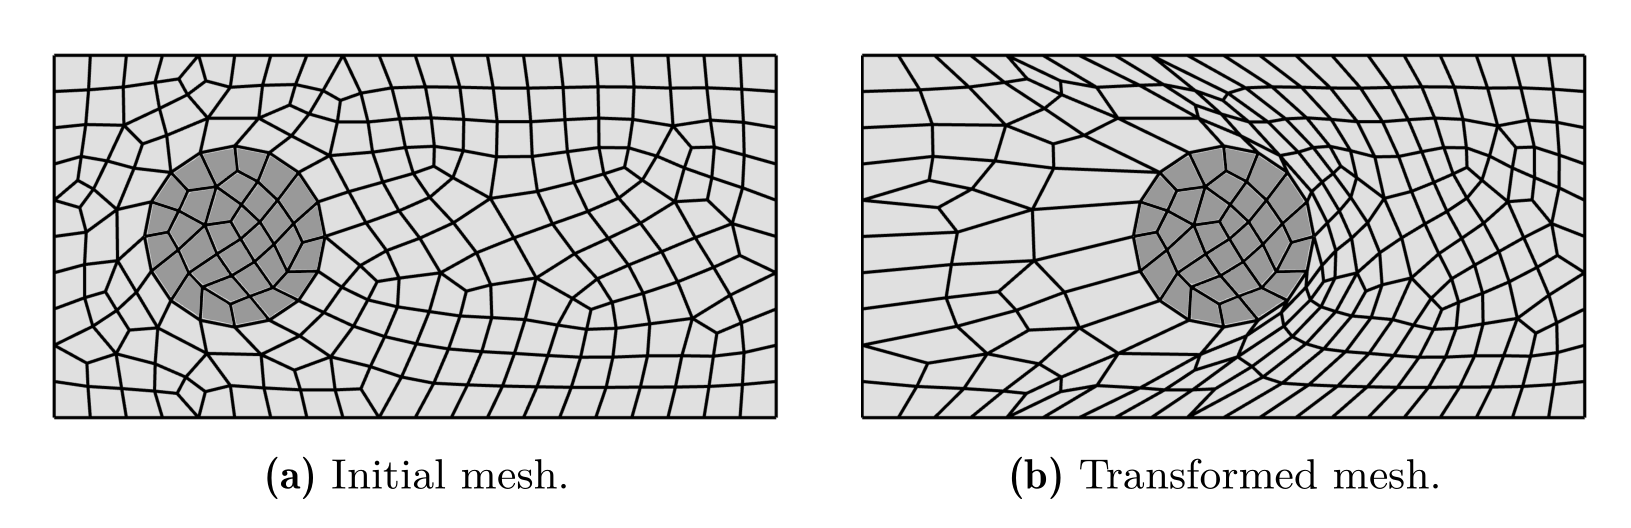
\includegraphics[width=0.95 \textwidth]{figures/transformed_mesh.png}
                \end{figure}
    \end{block}
\end{frame}


\begin{frame}{}

    \begin{block}{ Other problems of unstructured mesh }
        \begin{itemize}
            \item Unstructured mesh is difficult to parallelize
            \item Cannot handle smooth boundaries. Some application may actually require smooth boundaries (shape optimization etc).
        \end{itemize}
    \end{block}
    \begin{figure}
        \centering
        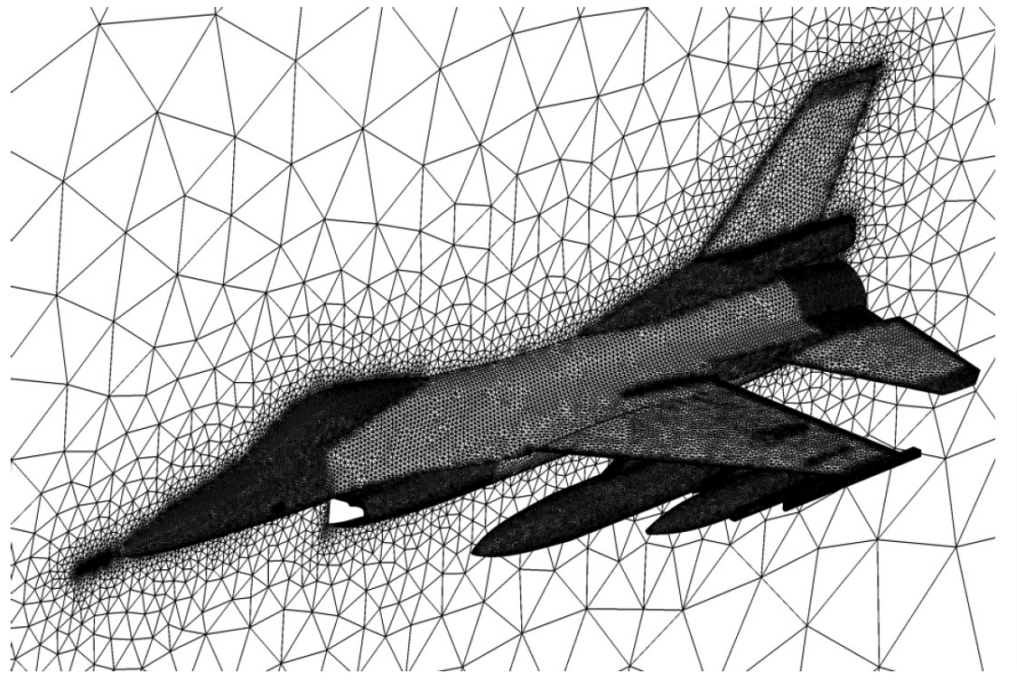
\includegraphics[width=0.45 \textwidth]{figures/unstructured_mesh_f16.png}
    \end{figure}
\end{frame}

\begin{frame}{Ways to solve this problem}
    \begin{itemize}
        \item Change the geometry.
            \begin{enumerate}
                \item Time-dependent mesh elements on moving domains.
                \item Delete and add nodes when necessary.
                \item Full re-mesh generation.
                \item Probably many more clever methods $\ldots$
            \end{enumerate}
        \item Utilize the geometry instead of modifying it
            \begin{enumerate}
                \item Method that can handle smooth boundaries.
                \item Do some smart transformations
            \end{enumerate}
    \end{itemize}
    \begin{block}{Question}
        \textbf{How do you approach this problem?}
    \end{block}

\end{frame}

\begin{frame}{Cut finite element method}
     Method to solve PDE's with moving domains on a unfitted mesh!
                \begin{figure}
                    \centering
                    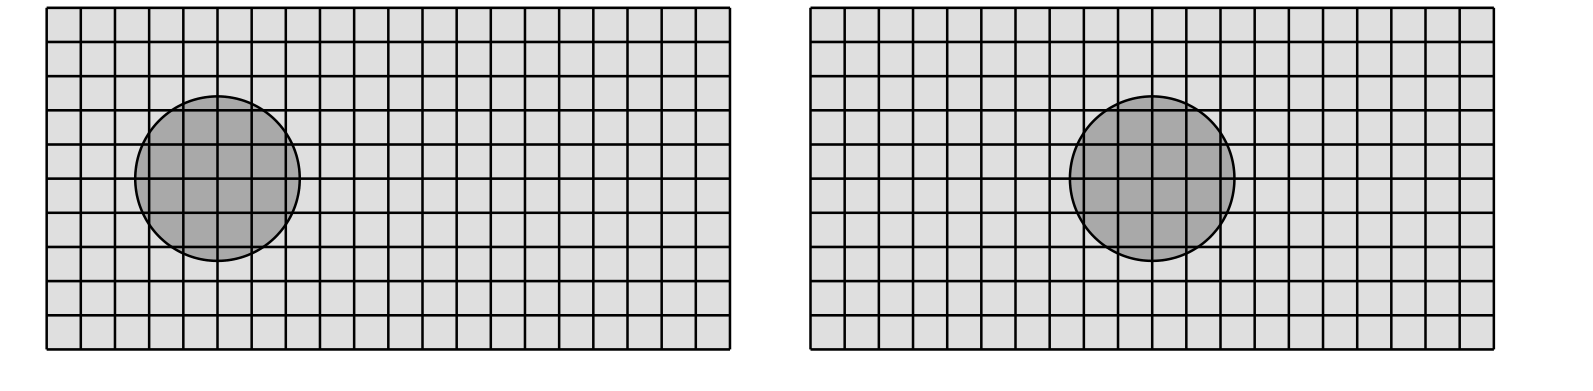
\includegraphics[width=0.95 \textwidth]{figures/transformed_mesh_unfitted.png}
                \end{figure}
    \begin{block}{  }
        \begin{itemize}
            \item Here we considering an smooth boundary $\Gamma $ in $C^2$
            \item No re-meshing on moving domains, only new configuration of cut cells.
            \item Potential to handle very complex geometries
        \end{itemize}
    \end{block}

\end{frame}

\begin{frame}{Example of complex domains}

        \begin{figure}
            \centering
            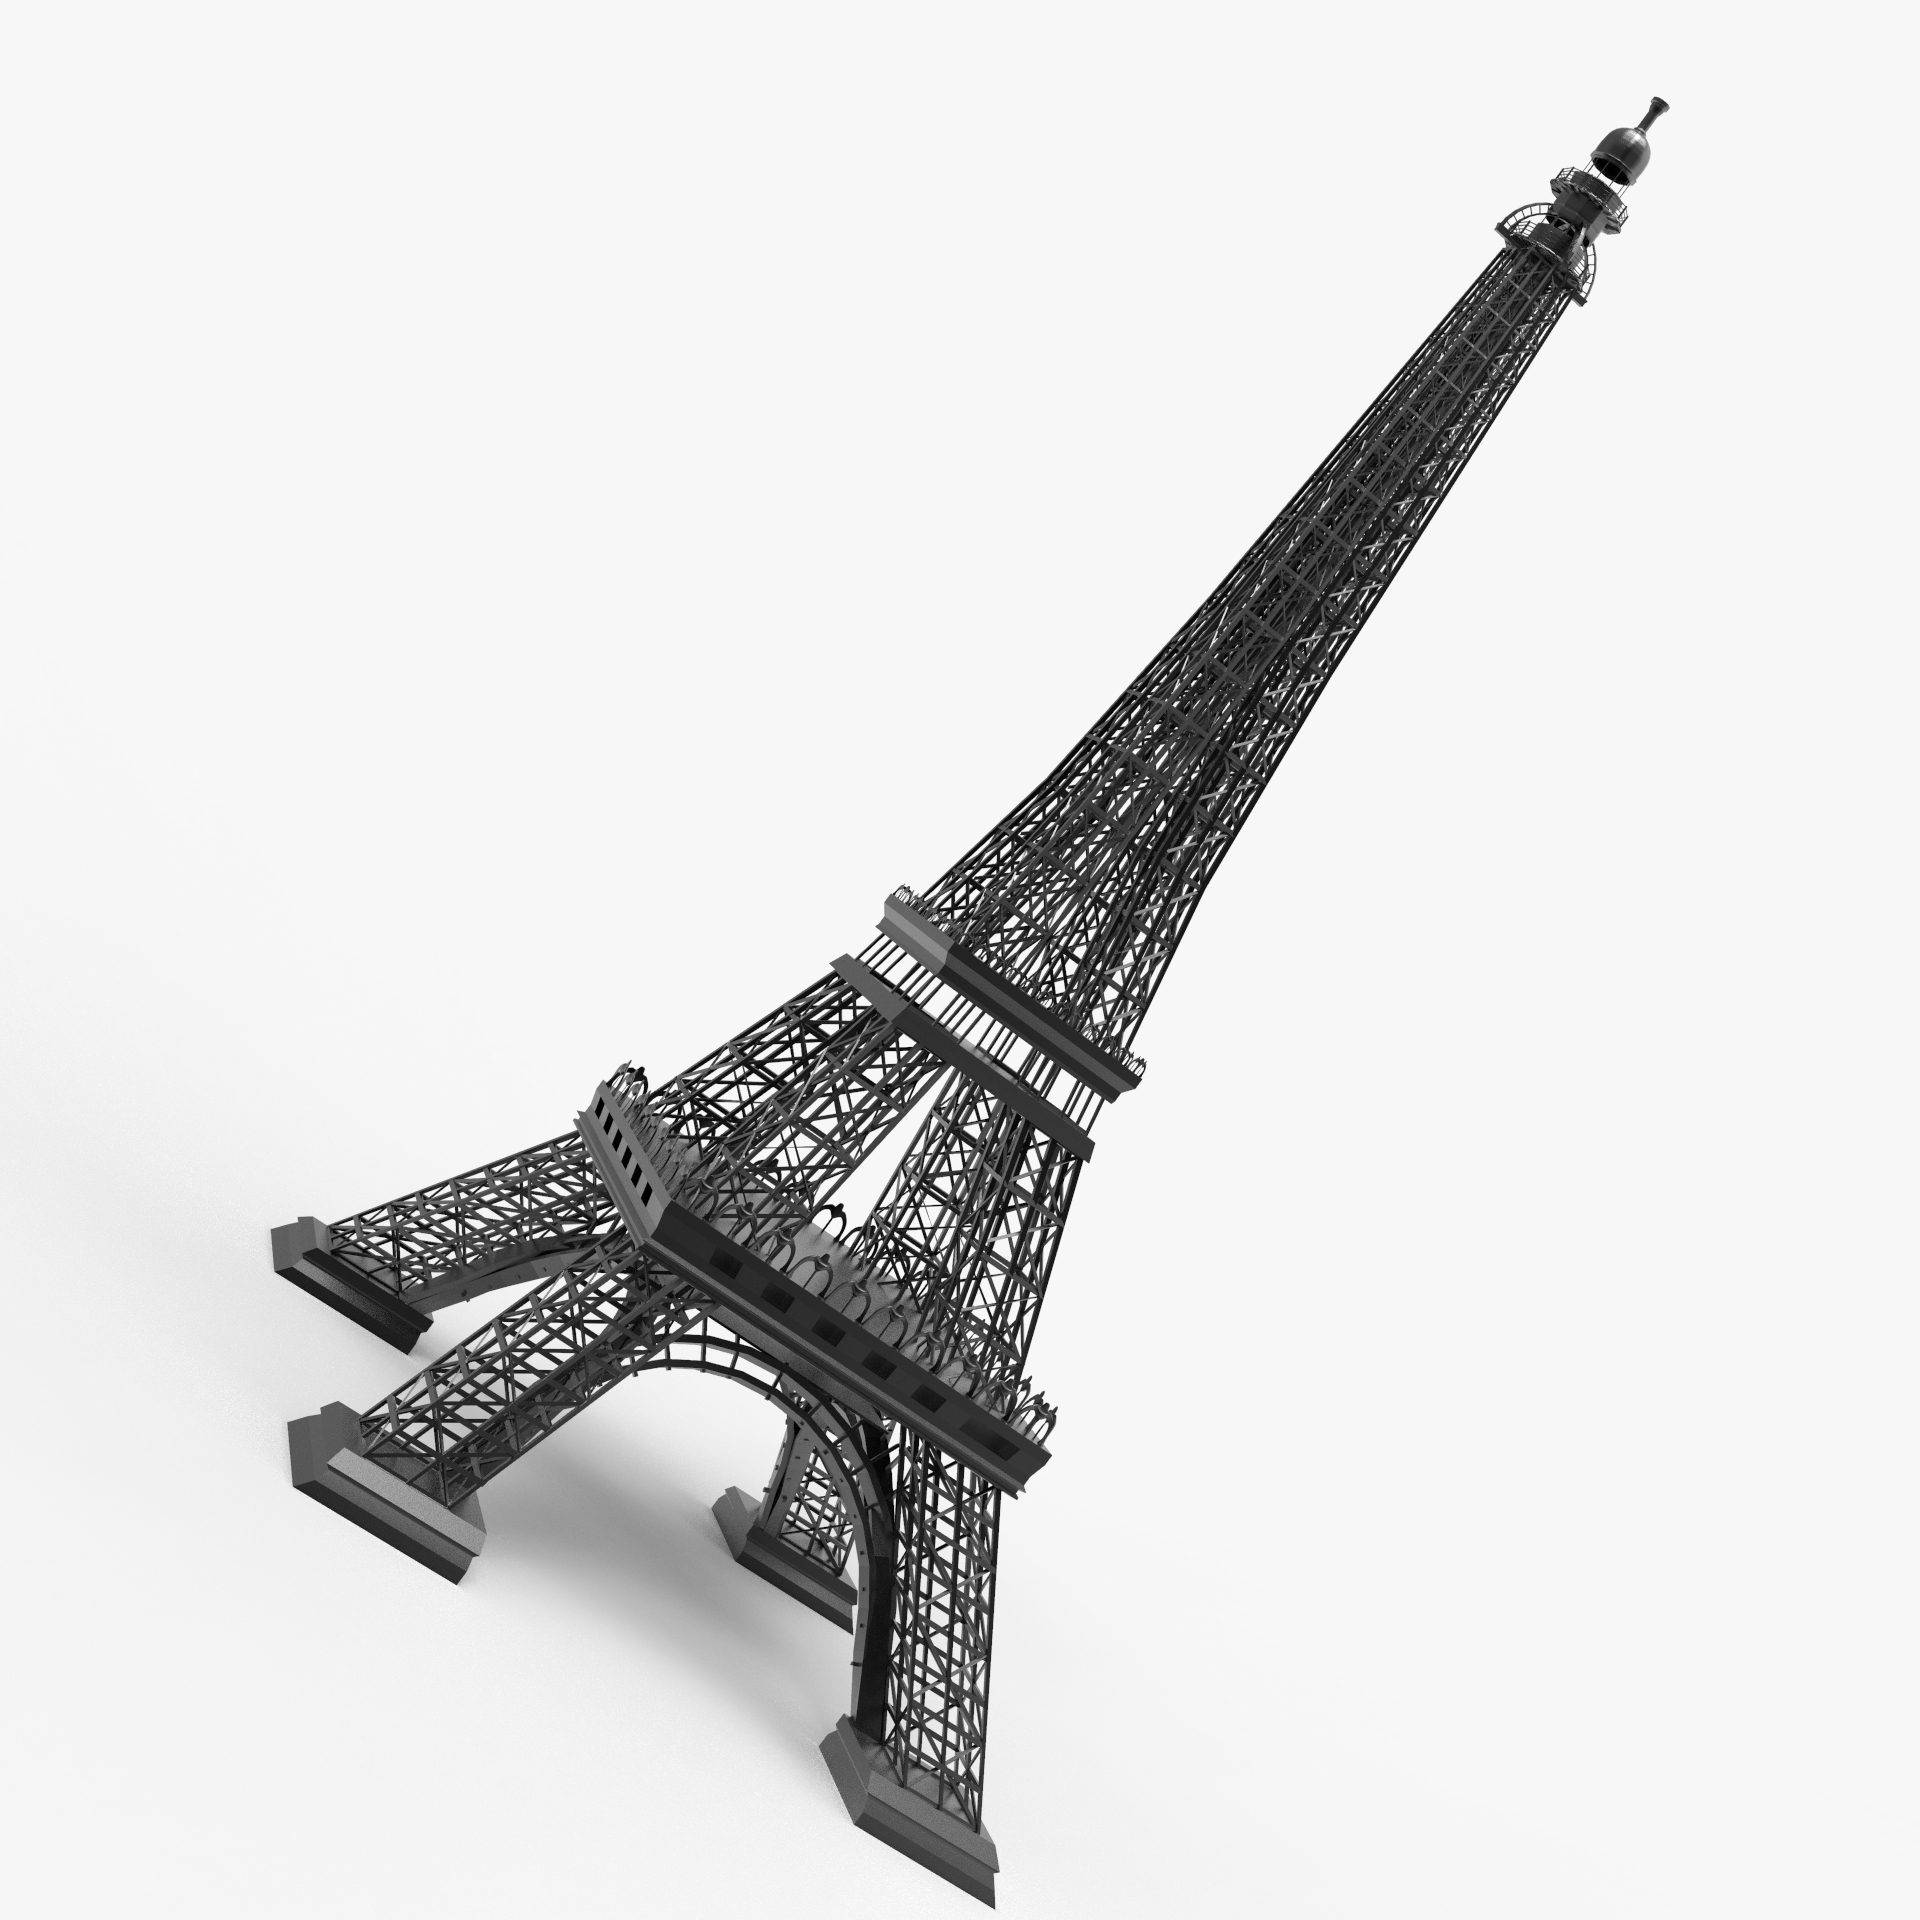
\includegraphics[width=6cm]{figures/eiffel_tower.jpg}
        \end{figure}

\end{frame}
\begin{frame}{Navier-Stokes on moving domains}

        \begin{figure}
            \centering
            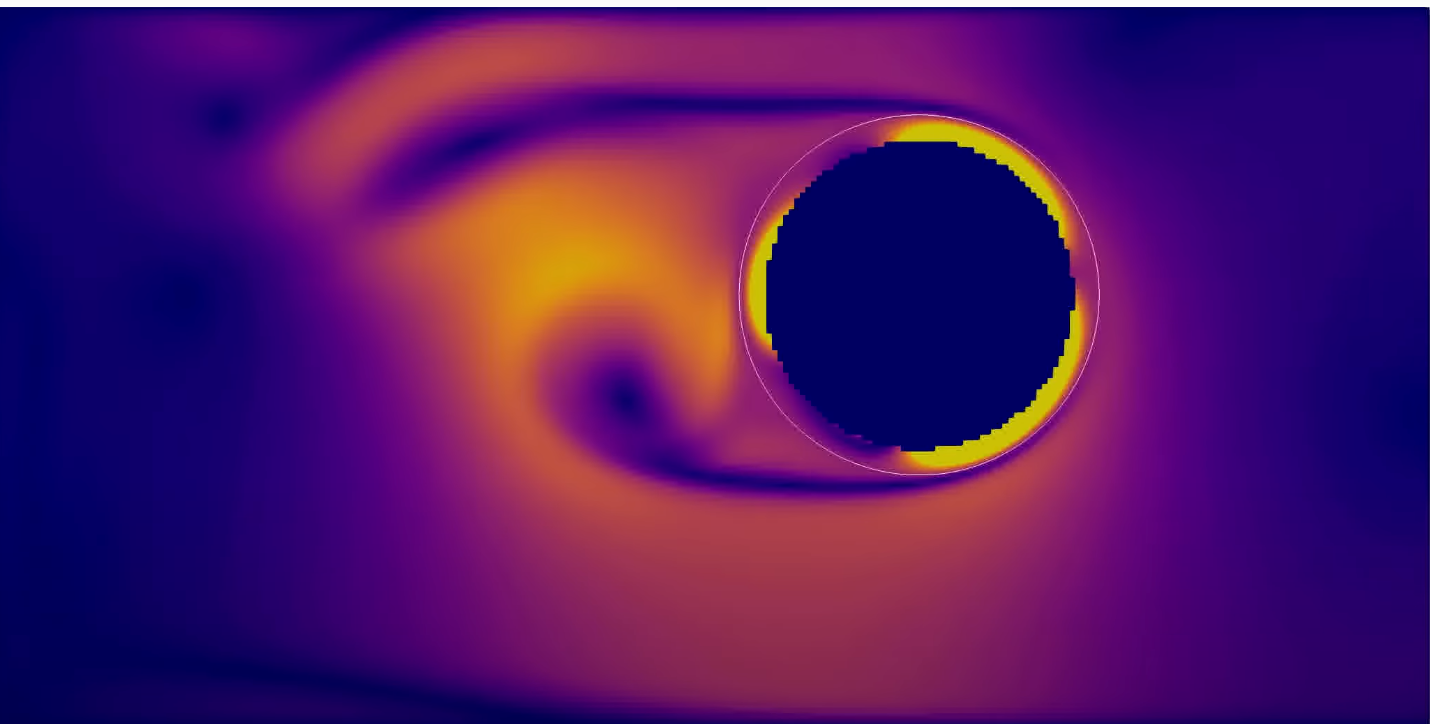
\includegraphics[width=8cm]{figures/navier_stokes.png}
        \end{figure}

    \href{https://www.youtube.com/watch?v=9dYdPOgPDUI&ab_channel=SigmundEggenHolm}{Link} to video
\end{frame}
\begin{frame}{Computational Domains}
    \begin{block}{}
        \begin{figure}
            \centering
            \parbox{5cm}{
                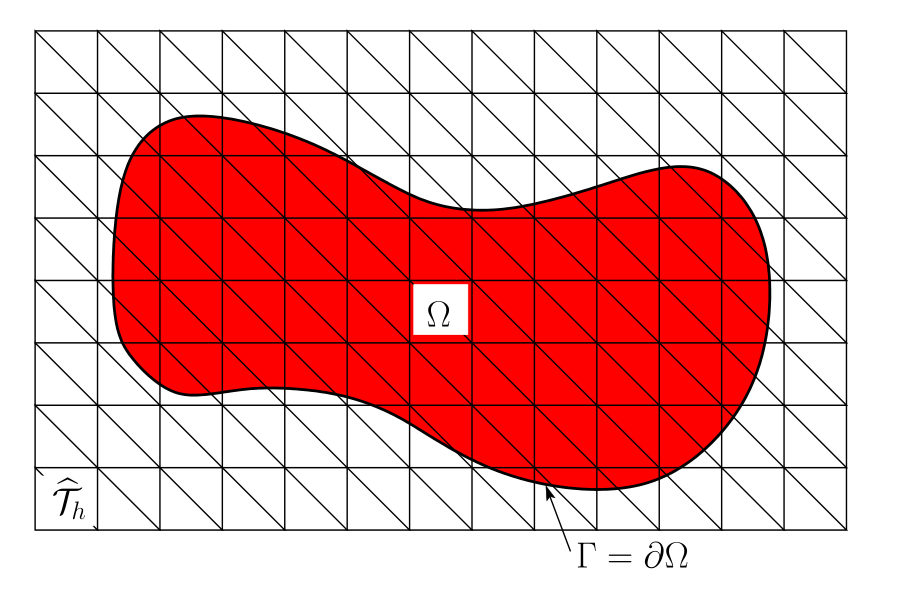
\includegraphics[width=4.5cm]{figures/physical_domain.png}
                \caption{Physical domain}
            \label{fig:2figsA}}
            \qquad
            \begin{minipage}{5cm}
                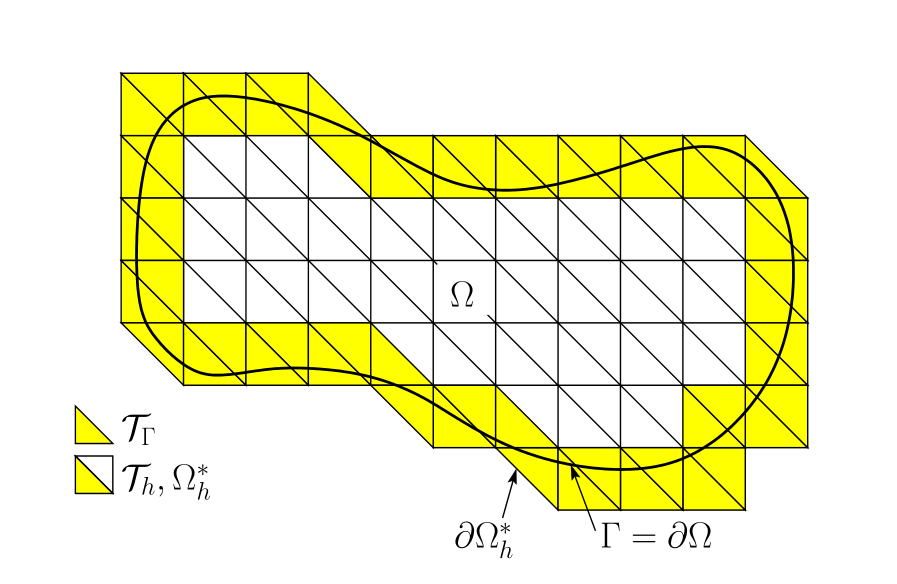
\includegraphics[width=4.5cm]{figures/minimal_subset.png}
                \caption{Cut cells}
                \label{fig:2figsB}
            \end{minipage}
        \end{figure}
        \begin{itemize}
            \item We define a background mesh $\widetilde{\mathcal{T} }_{h}$
            \item An active submesh $\mathcal{T} _{h} \subset \widetilde{\mathcal{T} _{h}}$ containing physical domain $\Omega $.
            \item Cut cells $ \mathcal{T} _{\Gamma} \subset \mathcal{T} _{h} $ is the mesh elements that intersects with the boundary $\Gamma  $.
        \end{itemize}
    \end{block}
\end{frame}

\begin{frame}{Constructing the method}
        \begin{columns}
        \begin{column}{0.5\textwidth}
        \begin{figure}
            \centering
            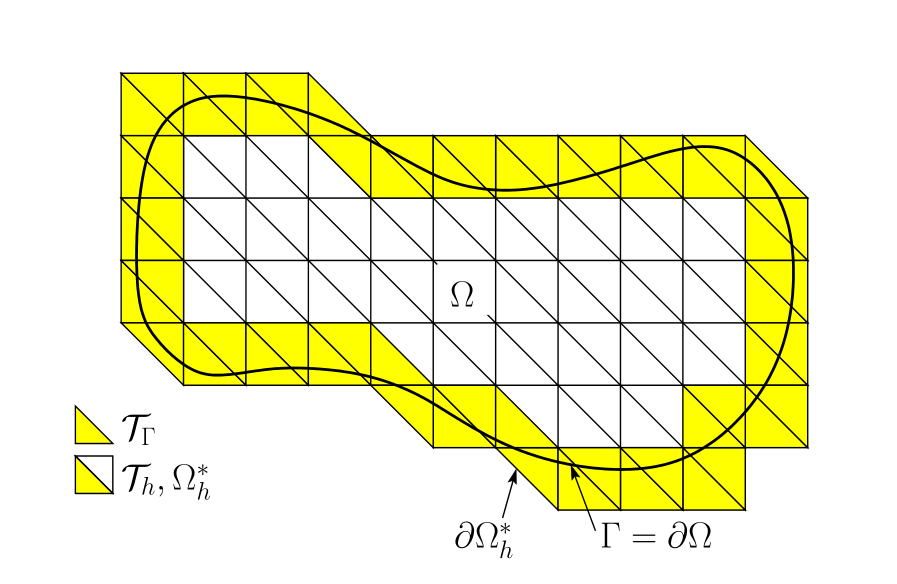
\includegraphics[width=8.2cm]{figures/minimal_subset.png}
        \end{figure}
        \end{column}

        \begin{column}{0.5\textwidth}
        \begin{block}{Observation}
            \begin{enumerate}
                \item The interior is pretty nice to deal with.
                \item The boundary must be parametrized somehow.
                    \begin{itemize}
                        \item Level-set functions $\varphi ( x) = 0 $ is one way.
                        \item Splines is also possible
                    \end{itemize}
                \item How do we deal with Dirichlet conditions?
                \item How do we deal with elements with "bad" cuts?
                \item Can we show that the problem is still well-posed?
            \end{enumerate}
        \end{block}
        \end{column}
        \end{columns}

\end{frame}

\begin{frame}{Recall Poisson problem }
        Recall the formulation \( ( \nabla u, \nabla v)_\Omega - ( \partial _{n} u, v)_{\Gamma } = ( f,v)_{\Omega }
        \)
        \begin{block}{Problem}
            \begin{itemize}
                \item
            Dirichlet conditions is embedded in the function space, \( V_{g} = \left\{ v \in H^{1 }( \Omega )   \mid  u = g \text{ on }  \Gamma   \right\} \)
        \item But is difficult to handle when $\Gamma $ is smooth.
            \end{itemize}
        \end{block}

        \begin{block}{Can we impose the Dirichlet conditions naturally?}
            Yes! We add a penalty on the boundary $ \mu (u-g,v )_{\Gamma }  $,
            \[
            ( \nabla u, \nabla v)_\Omega - ( \partial _{n} u, v)_{\Gamma }+ \mu (u,v )_{\Gamma } = ( f,v)_\Omega  + \mu (g,v )_{\Gamma }.
            \]
            For symmetry we can also add $(u-g , \partial _{n} v)_{\Gamma } $,\[
            ( \nabla u, \nabla v)_\Omega - ( \partial _{n} u, v)_{\Gamma } + (-u , \partial _{n} v)_{\Gamma }+ \mu (u,v )_{\Gamma } = ( f,v)_\Omega  + \mu (g,v )_{\Gamma }+ (-g , \partial _{n} v)_{\Gamma }.
            \]

        \end{block}
\end{frame}
\begin{frame}{Poisson formulation on a smooth boundary   }

    Recall that $\mathcal{T}_{h} $ is the active mesh, that is, all trianges intersection with the interior of the domain $\Omega$.
        \begin{block}{Definitions}
            Let $V_{h} := \mathcal{P}^{k}( \mathcal{T}_{h} )\cap C^{0}( \Omega )   $.We denote the bilinear form  $a_{h}:V_{h} \times V_{h} \to \mathbb{R} $ and the linear form  $l_{h}: V_{h} \to \mathbb{R} $ to be,\[
                \begin{split}
                a_{h}( u,v)&  :=  ( \nabla u, \nabla v)_\Omega - ( \partial _{n} u, v)_{\Gamma } - (u , \partial _{n} v)_{\Gamma }+ \mu (u,v )_{\Gamma }  \\
                l_{h} ( v) & :=( f,v)_\Omega  + \mu (g,v )_{\Gamma } - (g , \partial _{n} v)_{\Gamma }
                \end{split}
            \]

        \end{block}
        \begin{block}{Problem Statement}
            We want to find a $u \in V_{h} $ s.t. $a_{h}( u,v) = l_{h}( v)  \quad \forall v \in V_{h} $.
        \end{block}
\end{frame}

\begin{frame}{ Recall Lax Milgram }

    \begin{theorem}[ ]

        $a_{h}( u,v) = l_{h}( v)  $ well-posed if both of these statements holds;
        \begin{itemize}
            \item The bilinear form is bounded,
                \[
                      \abs{a_{h}( v,w)  }    \le C_{1} \| v \|_{a_{h}  }^{  }  \| w \|_{a_{h}  }^{  } \quad \forall v,w  \in V_{h}.
                \]
            \item The bilinear form is coercive (one-to-one), \[
           a_{h}( v,v) \ge  C_{2} \| v \|_{ a_{h} }^{  2} \quad \forall v \in V_{h}.
            \]
        \end{itemize}
    \end{theorem}
\end{frame}

\begin{frame}{Is the new system well-posed?  }

    \begin{itemize}
        \item The Dirchlet conditions problem is in good shape for smooth domains!
        \item But from basic FEM theory it is now necessarry to apply  \[
h^{\frac{1}{2}} \| \partial _{n} v \|_{ \Gamma \cap T  }^{  } \le C \| v  \|_{ \Omega \cap T      }^{  }
        \]
        to obtain well-posedness!
        \item But what about integration on very bad cut elements?
            \begin{itemize}
                \item The relation between length $  \abs{F\cap \Omega  } $ and volume $ \abs{T\cap \Omega  } $ is very different on cut elements, thus, the norm is unbounded if the cut is bad.
            \end{itemize}
    \end{itemize}

\end{frame}


\begin{frame}{The problem with the bad cuts}
        \begin{columns}
        \begin{column}{0.5\textwidth}
    \begin{figure}
        \centering
        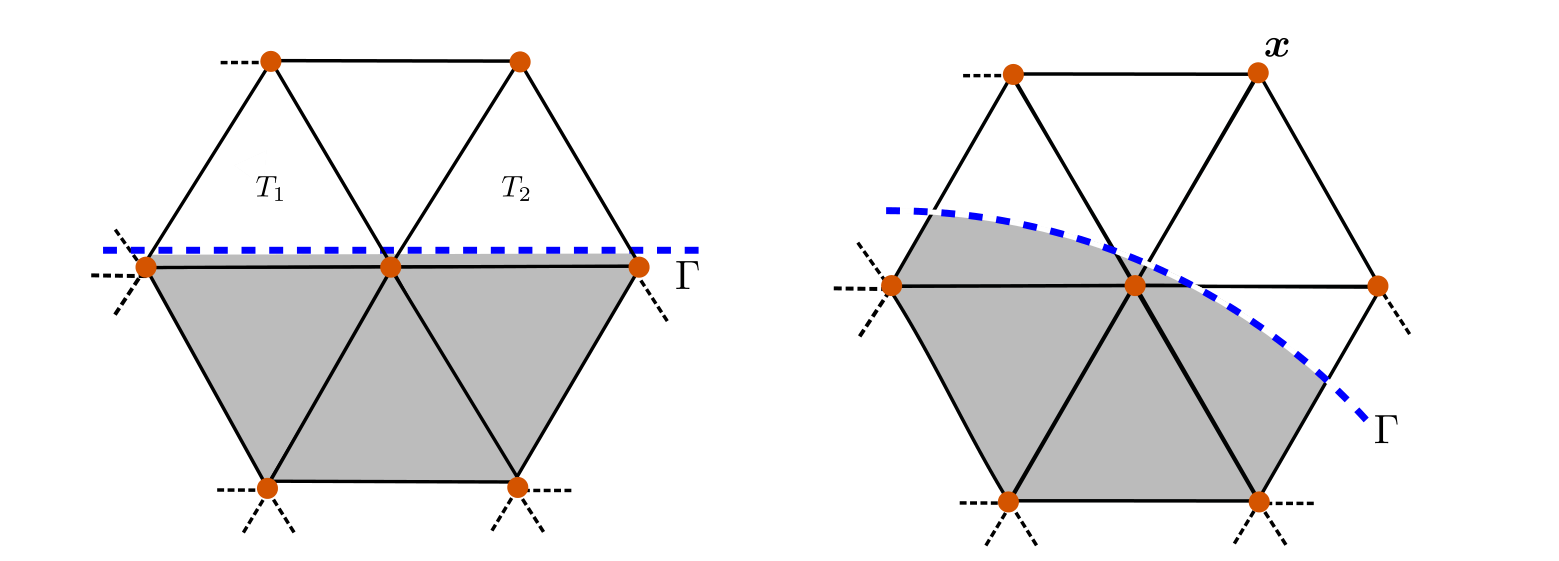
\includegraphics[width=8.8cm]{figures/bad_cuts.png}
    \end{figure}
        \end{column}

        \begin{column}{0.5\textwidth}
    \begin{block}{Observation}
        \begin{itemize}
            \item Bad cuts makes it hard to justify length $F\cap \Omega$  vs area $\abs{T\cap \Omega } $. Thus, the necessarry \[
h^{\frac{1}{2}} \| \partial _{n} v \|_{ \Gamma \cap T  }^{  } \le C \| v  \|_{ \Omega \cap T      }^{  }
            \]
            become unbounded. Hence, the system is ill-conditoned.
            \item  We are forced to extend the norm s.t. \[
h^{\frac{1}{2}} \| \partial _{n} v \|_{ \Gamma \cap T  }^{  } \le C \| v  \|_{  T      }^{  }
            \]
            But we are integrating outside of our domain :(

        \end{itemize}
    \end{block}
        \end{column}
        \end{columns}
\end{frame}

\begin{frame}{Ghost penalty}

    The solution of the inverse estimate problem is simple! We add a \textbf{ghost penalty} $g_{h}( u,v) $ to handle the bad cuts as an regularization!
    $$h^{\frac{1}{2}} \| \partial _{n} v \|_{ \Gamma \cap T  }^{  } \le C \| v  \|_{  T      }^{  }+ g_{h}( u,v) $$
    The goal is to regulate the ill-conditioned problem!
    \begin{itemize}
        \item We give it the necessarry assumptions for Lax-Milgram to hold!
        \item Same strategy is used to to obtain optimal convergence!
        \item We then engineer the $g_{h}$ given the assumptions!
    \end{itemize}

    Hence, we end up with this stabilized problem formulation

    \begin{block}{Stabilized Poission Problem}
        Let $A_{h}( u,v) := a_{h}( u,v) + g_{h}( u,v)   $.
            We want to find a $u \in V_{h} $ s.t.
            \[
            A_{h}( u,v) = l_{h}( v)  \quad \forall v \in V_{h}
            \]
    \end{block}
\end{frame}

\begin{frame}{ The reality is more nasty}

    \begin{figure}
        \centering
        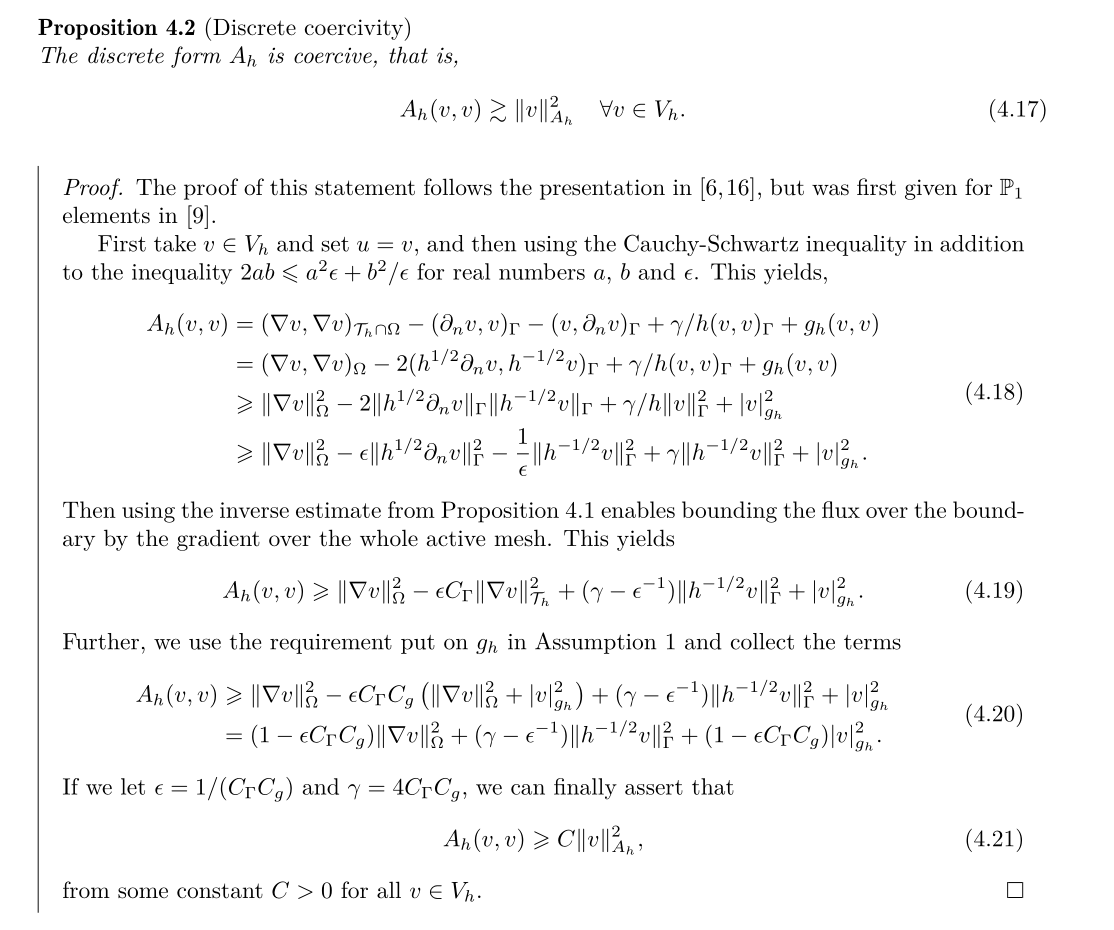
\includegraphics[width=8.5cm]{figures/reality.png}
    \end{figure}

\end{frame}
\begin{frame}{ }

    \begin{block}{But I hope at least you have learned something new :) }
    \end{block}

\end{frame}

\begin{frame}{ }

    \begin{block}{Questions? }
    \end{block}

\end{frame}
